\documentclass[12pt]{article}
\usepackage{times,fullpage,xspace,fancyhdr,url,graphicx,xspace}
\usepackage[usenames,dvipsnames]{color}
\usepackage[utf8]{inputenc}
\usepackage[T1]{fontenc}
\usepackage{amsmath}
\usepackage[pdftex,colorlinks=true,urlcolor=black,linkcolor=black,citecolor=black,bookmarksopen=false,bookmarksnumbered=true,pdfstartview=FitH,pdfpagelabels]{hyperref}
\hypersetup{
	pdftitle={Laws of the RoboCup Small Size League 2013},
	pdfauthor={Small Size League Technical Committee},
}


\setlength{\parindent}{0pt}
\setlength{\parskip}{12pt plus 6pt minus 3pt}
\widowpenalty=10000
\clubpenalty=10000

\pagestyle{fancy}
\lhead{}
\chead{}
\rhead{}
\lfoot{}
\cfoot{}
\rfoot{}

\renewcommand{\headrulewidth}{0.4pt}
\renewcommand{\footrulewidth}{0.4pt}

\def\sectionautorefname{Law}
\def\subsectionautorefname{Subsection}

\begin{document}

\setcounter{page}{1}
\pagenumbering{roman}

\title{Laws of the RoboCup Small Size League 2013}
\author{Small Size League Technical Committee}

\maketitle

\vfill

\tableofcontents

\section*{Notes}
Male and Female---References to the male gender in the Laws with respect to referees, assistant referees, team members and officials are for simplification and apply to both males and females.

\thispagestyle{fancy}

\clearpage

\cfoot{\thepage}
\setcounter{page}{1}
\pagenumbering{arabic}

\section{The Field of Play}\label{sec:field-of-play}

\subsection{Dimensions}
The field of play must be rectangular.
\added{Teams have the option of choosing to play on one of two sizes of fields: }
\begin{enumerate}
\item \textbf{\added{Single-size field}}, of size 6050\,mm$\times$ 4050\,mm
\item \textbf{\added{Double-size field}}, of size 8090\,mm$\times$ 6050\,mm
\end{enumerate}
The dimensions include boundary lines.
Dimensions of the field, goals, and special field areas are in millimetres and
are shown in \autoref{fig:single_size_field} (single-size field) and
\autoref{fig:double_size_field}(double-size field).

\begin{figure}[ht] % ht = here / t = top / b = bottom
	\centering
	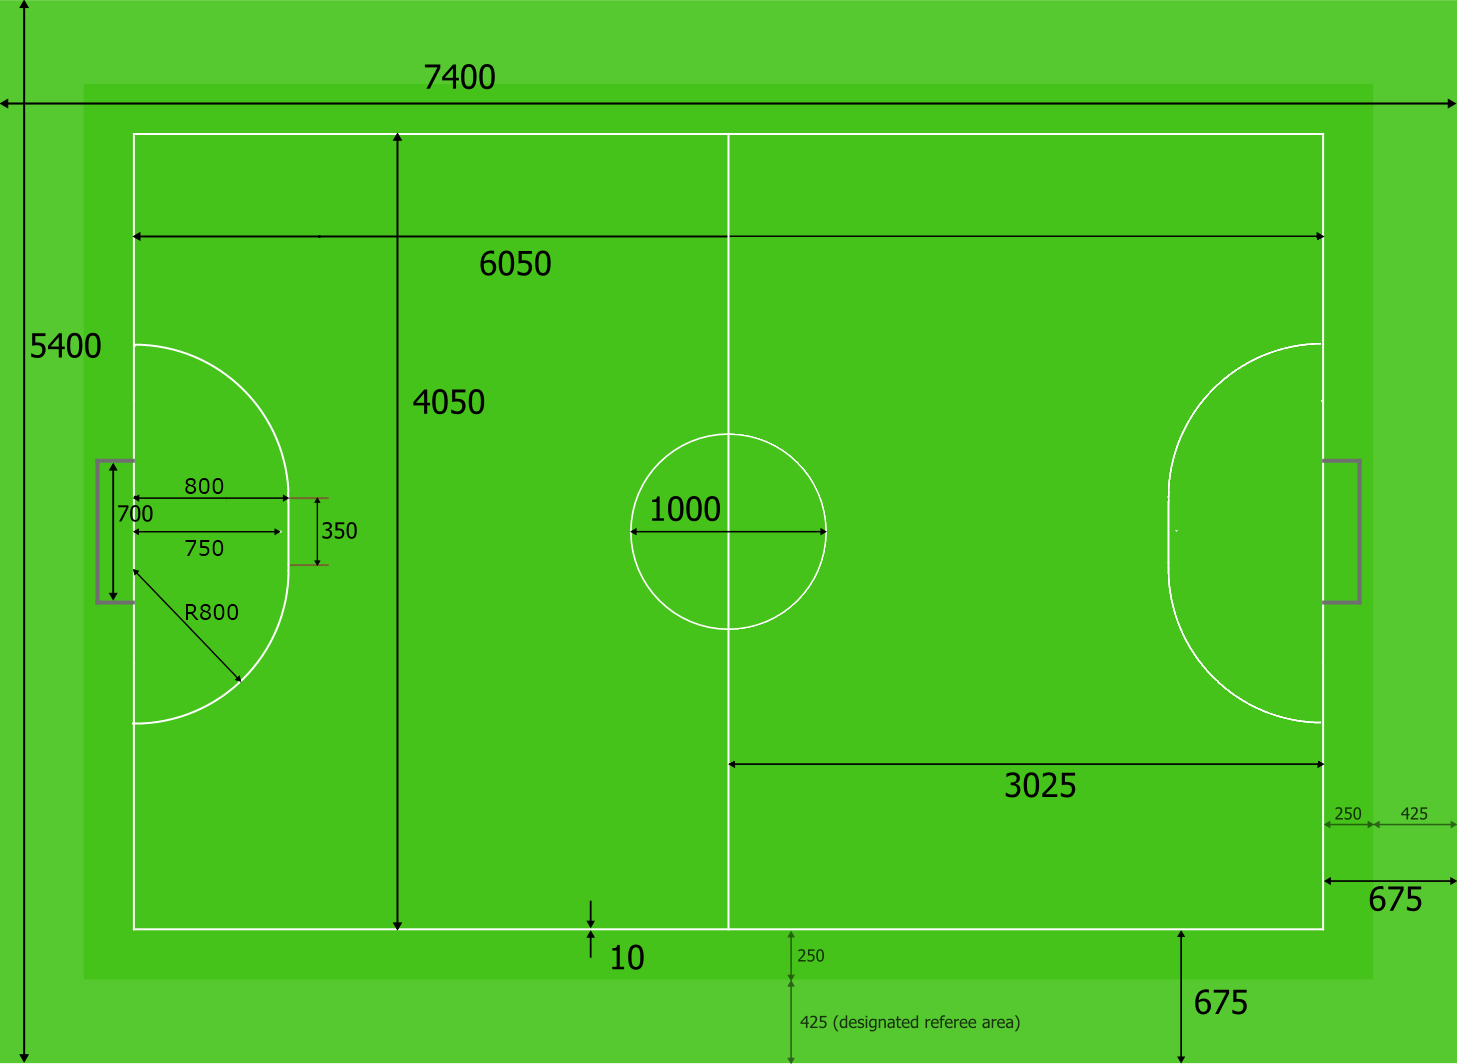
\includegraphics[width=0.8\columnwidth]{img/field_2012_drawing.png}
	\caption{The field dimensions of the single-size field}
	\label{fig:single_size_field}
\end{figure}

\begin{figure}[ht] % ht = here / t = top / b = bottom
	\centering
	\includegraphics[width=0.8\columnwidth]{img/double-size-field.png}
	\caption{The field dimensions of the double-size field}
	\label{fig:double_size_field}
\end{figure}

\added{
The rules in this rule book apply identically to both sizes of fields, unless otherwise explicitly mentioned.
Specifically, the following rules have differences in their application to the two field sizes:
}
\begin{enumerate}
\item \added{The number and length of timeouts in \autoref{subsec:duration-of-the-match-timeouts}}
\item \added{The robot speed limit during stoppage of play in \autoref{subsec:fouls-and-misconduct-disciplinary-sanctions}}
\end{enumerate}

\subsection{Field Surface}
The playing surface is green felt mat or carpet.
The floor under the carpet is level, flat, and hard.

The field surface will continue for 675\,mm beyond the boundary lines on all sides.
The outer 425\,mm of this runoff area are used as a designated referee walking area (see \autoref{sec:referee}).
At the edge of the field surface, a 100\,mm tall wall will prevent the ball and robots from running off the edge.

\subsection{Field Markings}
The field of play is marked with lines.
Lines belong to the areas of which they are boundaries.

The two longer sides are called touch boundaries.
The two shorter sides are called goal boundaries.

All lines are 10\,mm wide and painted white.

The field of play is divided into two halves by a halfway line.

The centre mark is indicated at the midpoint of the halfway line.
A circle with a diameter of 1000\,mm is marked around it.

\subsection{The Defence Area}
A defence area is defined at each end of the field as follows:

Two quarter circles with a radius of 800\,mm are drawn on the field of play.
These quarter circles are connected by a line parallel to the goal line.
The exact configuration is depicted in figure \ref{fig:sslfield}.

The area bounded by this arc and the goal line is the defence area.

\subsection{Penalty Mark}
Within each defence area a penalty mark is made 750\,mm from the midpoint between the goalposts and equidistant to them.
The mark is a 10\,mm diameter circle of white paint.

\subsection{Goals}
Goals must be placed on the centre of each goal boundary \added{and anchored
securely to the field surface}.

They consist of two 160\,mm vertical side walls joined at the back by a 160\,mm vertical rear wall.
The inner face of the goal has to be covered with an energy absorbing material such as foam to help absorb ball impacts and lessen the speed of deflections.
The goal walls, edges, and tops are white in color.

There is a round steel cross bar that runs across the top of the goalmouth and parallel to the goal line.
It is no larger than 10\,mm in diameter, but is sufficiently strong to deflect the ball.
The bottom of the bar is 155\,mm from the field surface, and the bar is dark in color to minimise interference with vision systems.
The top of the goal is covered in a thin net to prevent the ball from entering the goal from above.
It is attached securely to the cross bar and goal walls.

The distance between the side walls is 700\,mm \added{for the single-size field
and 1000\,mm for the double-size field, and the goal is 180\,mm deep}.
\removed{The goal is 180\,mm deep. The distance from the lower edge of the
crosswire to the playing surface is 150\,mm.}
The goal walls are 20\,mm thick \added{and touch the outer boundary of the field
at the goal line, but do not overlap or encroach on the field lines or the field}.

The floor inside the goal\removed{mouth} is the same as the rest of the playing surface.

\removed{Goals must be anchored securely to field surface.}

\begin{figure}[ht] % ht = here / t = top / b = bottom
	\centering
	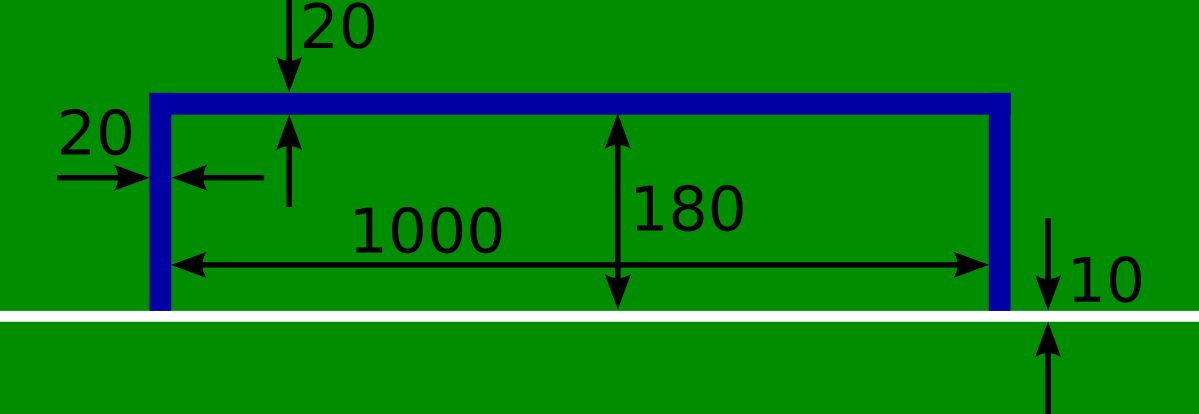
\includegraphics[width=0.5\columnwidth]{img/goal_detail.png}
	\caption{The Goal in detail}
	\label{fig:sslgoal}
\end{figure}

\subsection{Equipment Mounting Bar}
A mounting bar will be provided 4\,m above the field.
The bar will run above the midline of the field from goal to goal.
The bar should be mounted securely so that it does not swing or sway under a small external force, and it should not bend or twist significantly when the weight of typical video equipment is added.

\subsection{Shared Vision System}
Each field is provided with a shared central vision server and a set of shared cameras.
This shared vision equipment uses the community-maintained \textbf{SSL-Vision}\footnote{\url{http://codegooglecom/p/ssl-vision/}} software to provide localization data to teams via Ethernet in a packet format that is to be announced by the shared vision system developers before the competition.
Teams need to ensure that their systems are compatible with the shared vision system output and that their systems are able to handle the typical properties of real-world sensory data as provided by the shared vision system (including noise, latency, or occasional failed detections and misclassifications).

Besides the shared vision equipment, teams are \emph{not} allowed to mount their own cameras or other external sensors, unless specifically announced or permitted by the respective competition organisers.

The shared vision system in each field is maintained by one or more vision experts.
The procedure of selection of these experts will be announced by the competition organisers.
\autoref{app:vision-experts} describes the duties of the vision experts.

\subsection*{Decisions of the Small Size League Technical Committee}
\begin{enumerate}
\item
The local organising committee should aim to provide uniform, diffuse lighting conditions of approximately 500\,lux or brighter.
No special lighting equipment will necessarily be used to provide these conditions.
The brightness is not guaranteed nor expected to be fully uniform across the field surface.
Teams are thus expected to cope with the variations that will occur when using ambient lighting.
The organising committee will release details of the lighting arrangements to the competitors as early as practical.

\item
No kind of commercial advertising, whether real or virtual, is permitted on the field of play and field equipment (including the goal nets and the areas they enclose) from the time the teams enter the field of play until they have left it at half-time and from the time the teams re-enter the field of play until the end of the match.
In particular, no advertising material of any kind may be displayed inside the goals or walls.
No extraneous equipment (cameras, microphones, etc.) may be attached to these items.

\item
The specific color and texture of the surface is not specified and may vary from competition to competition (just as real soccer fields vary).
The surface underneath the carpet will be level and hard.
Examples of approved surfaces include: cement, linoleum, hardwood flooring, plywood, ping-pong tables and particle board; carpeted or cushioned surfaces are not allowed.
Every effort shall be made to ensure that the surface is flat; however, it is up to individual teams to design their robots to cope with slight curvatures of the surface.
\end{enumerate}

\section{The Ball}\label{sec:ball}

\subsection{Qualities and Measurements}
The ball is a standard orange golf ball.
It is:
\begin{itemize}
\item spherical
\item orange in color
\item approximately 46\,g in mass
\item approximately 43\,mm in diameter
\end{itemize}

\subsection{Replacement of a Defective Ball}
If the ball becomes defective during the course of a match:
\begin{itemize}
\item the match is stopped
\item the match is restarted by placing the replacement ball at the place where the first ball became defective
\end{itemize}

If the ball becomes defective whilst not in play at a kick-off, goal kick, corner kick, free kick, penalty kick, or throw-in:
\begin{itemize}
\item the match is restarted accordingly
\end{itemize}

The ball may not be changed during the match without the authority of the referee.
\section{The Number of Robots}\label{sec:number-of-robots}

\subsection{Robots}
A match is played by two teams, each consisting of not more than six robots, one of which may be the goalkeeper.
Each robot must be clearly numbered so that the referee can identify them during the match.
The goalkeeper must be designated before the match starts.
A match may not start unless both teams have at least one robot.

\subsubsection{Interchange}\label{subsubsec:number-of-robots-interchange}
Robots may be interchanged.
There is no limit on the number of interchanges.

\subsubsection{Interchange Procedure}
To interchange a robot, the following conditions must be observed:
\begin{itemize}
\item interchange can only be made during a stoppage in play,
\item the referee is informed before the proposed interchange is made,
\item the interchange robot enters the field of play after the robot being replaced has been removed,
\item the interchange robot enters the field of play at the halfway line.
\end{itemize}

\subsubsection{Changing the Goalkeeper}
Any of the other robots may change places with the goalkeeper, provided that:
\begin{itemize}
\item the referee is informed before the change is made of which robot will be the new goalie
\item the change is made during a stoppage in the match
\item the referee indicates the number of the new goalie, which is sent by communication link to the teams
\end{itemize}

\subsection*{Decisions of the Small Size League Technical Committee}
\begin{enumerate}
\item
Each team must have a single designated robot handler to perform interchange and robot placing when required.
No other team members can encroach upon the area immediately surrounding the field.
Movement of robots by the handler is not allowed.
\end{enumerate}

\section{The Robotic Equipment}\label{sec:robotic-equipment}

\subsection{Safety}
A robot must not have in its construction anything that is dangerous to itself, another robot, or humans.

\subsection{Shape}
A robot must fit inside a 180\,mm diameter cylinder and have a height of 150\,mm or less.
Additionally, a robot's top area must adhere to the Standard Pattern size and surface constraints as described further below in this Law.

\begin{figure}[ht] % ht = here / t = top / b = bottom
	\centering
	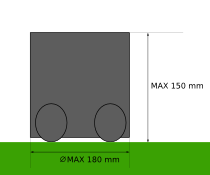
\includegraphics[width=0.5\columnwidth]{img/robot_size.png}
	\caption{The maximum robot dimensions}
	\label{fig:robotdimension}
\end{figure}

\subsection{Locomotion}
Robot wheels (or other surfaces that contact the playing surface) must be made of a material that does not harm the playing surface.

\subsection{Wireless Communication}
Robots can use wireless communication to computers or networks located off the field.

\subsection{Team Color}
Before a game, each of the two teams has a color assigned, namely yellow or blue.
All teams must be able to be either yellow or blue color.
The assigned team color is used as the centre marker color for all of the team's robots.
The detailed layout of the markers is described in \autoref{subsec:robotic-equipment-standard-pattern}.

\subsection{Standard Pattern}\label{subsec:robotic-equipment-standard-pattern}
All participating teams must adhere to the given operating requirements of the shared vision system (also see \autoref{sec:field-of-play}).
In particular, teams are required to use a certain set of standardized colors and patterns on top of their robots.

To ensure compatibility with the standardized patterns for the shared vision system, all teams must ensure that all robots have a flat surface with sufficient space available on the top side.
The color of the robot top must be black or dark grey and have a matte (non-shiny) finish to reduce glare.
The SSL-Vision standard pattern is guaranteed to fit within a circle of radius 85\,mm that is linearly cut off on the front side of the robot to a distance of 55\,mm from the centre, as shown in \autoref{fig:robothat}.
Teams must ensure that their robot tops fully enclose this area.

\begin{figure}[ht] % ht = here / t = top / b = bottom
	\centering
	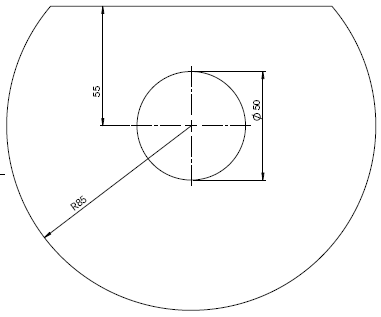
\includegraphics[width=0.8\columnwidth]{img/robot_hat.png}
	\caption{The Minimum Robot Top Area}
	\label{fig:robothat}
\end{figure}

The standard pattern to be used by all teams at RoboCup \removed{2012} is shown in \autoref{fig:stdpattern}.
Note that the organisers reserve the right to change this pattern at any time, if required.
Teams must therefore make sure to still adhere to the standard robot top area size as outlined in \autoref{fig:robothat}.

\begin{figure}[ht] % ht = here / t = top / b = bottom
	\centering
	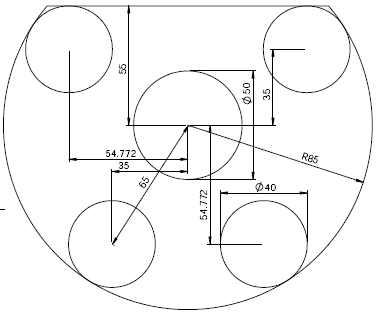
\includegraphics[width=0.8\columnwidth]{img/standard_pattern2010.png}
	\caption{The Standard Pattern}
	\label{fig:stdpattern}
\end{figure}

Each robot must use the standardized pattern with a unique color assignment selected from a standardized set of possible color combinations.
No two robots are allowed to use the same color assignment.
The centre dot color determines the team and is either blue or yellow.
Standardized colored paper or cardstock for all required colors will be provided at the competition.
The set of legal color assignments is shown in \autoref{fig:stdcolors}.
Note that the organisers reserve the right to change these color assignments at any time, if required.

\begin{figure}[ht] % ht = here / t = top / b = bottom
	\centering
	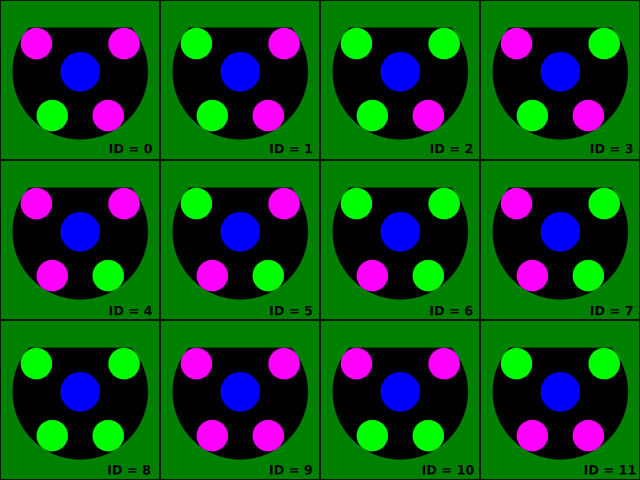
\includegraphics[width=1.0\columnwidth]{img/standard_colors2010.png}
	\caption{The Standard Color Assignments}
	\label{fig:stdcolors}
\end{figure}

Teams are encouraged to select color assignments with IDs 0--7 because they have been experimentally found more stable, as there is no risk that the back two dots ``color-bleed'' into each other.

\subsection{Autonomy}
The robotic equipment is to be fully autonomous.
Human operators are not permitted to enter any information into the equipment during a match, except at half time or during a time-out.

\subsection{Dribbling}
Dribbling devices that actively exert backspin on the ball, which keep the ball in contact with the robot are permitted under certain conditions.
The spin exerted on the ball must be perpendicular to the plane of the field.
Vertical or partially vertical dribbling bars, also known as side dribblers, are not permitted.
The use of dribbling devices is also restricted as per \autoref{sec:fouls-and-misconduct}, Indirect Free Kicks.

\begin{figure}[ht]
	\centering
	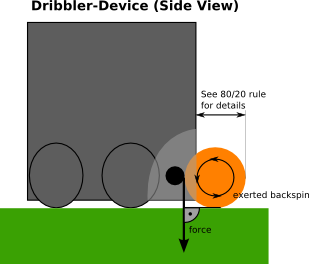
\includegraphics[width=0.5\columnwidth]{img/dribblers_1.png}
	\caption{How a dribbler may work (check \autoref{fig:20-rule} for further detail on the 20\% rule)}
	\label{fig:dribblers}
\end{figure}

\subsection{Infringements/Sanctions}
For any infringement of this Law:

\begin{itemize}
\item play need not be stopped
\item the robot at fault is instructed by the referee to leave the field of play to correct its equipment
\item the robot leaves the field of play when the ball next ceases to be in play
\item any robot required to leave the field of play to correct its equipment does not re-enter without the referee's permission
\item the referee checks that the robot's equipment is correct before allowing it to re-enter the field of play
\item the robot is only allowed to re-enter the field of play when the ball is out of play
\end{itemize}

A robot that has been required to leave the field of play because of an infringement of this Law and that enters (or re-enters) the field of play without the referee's permission is cautioned and shown the yellow card.

\subsection{Restart of Play}
If play is stopped by the referee to administer a caution:

\begin{itemize}
\item the match is restarted by an indirect free kick taken by a robot of the opposing side, from the place where the ball was located when the referee stopped the match
\end{itemize}

\subsection*{Decisions of the Small Size League Technical Committee}
\begin{enumerate}
\item
Participants using wireless communications shall notify the local organising committee of the method of wireless communication, power, and frequency.
The local organising committee shall be notified of any change after registration as soon as possible.

In order to avoid interference, a team should be able to select from two carrier frequencies before the match.
The type of wireless communication shall follow legal regulations of the country where the competition is held.
Compliance with local laws is the responsibility of the competing teams, not the RoboCup Federation.
The type of wireless communication may also be restricted by the local organising committee.
The local organising committee will announce any restrictions to the community as early as possible.

\item
Kicking devices are permitted.

\item
Metal spikes and Velcro are specifically prohibited for the purpose of locomotion.

\item
Bluetooth wireless communication is not allowed.

\item
Official colors will be provided by the organising committee.
Teams must use the official colors unless both teams agree not to.

\item
Adhesives such as glue or tape may not be used for the purpose of ball control or to construct dribblers.
Dribbling devices which use such an adhesive to affix the ball to a robot are considered a violation of \autoref{sec:fouls-and-misconduct}, Decision 4, by ``removing all of the degrees of freedom of the ball''.
In addition, the use of adhesives for any purpose on the robot which results in residue left on the ball or field, is considered as damage and sanctioned as per \autoref{sec:fouls-and-misconduct}.

\item
A rules check will be performed on all robots at the competition prior to the first match.
Any team's robot which is found to violate a rule must be modified to be compliant before it can participate in matches.

\end{enumerate}
\section{The Referee}\label{sec:referee}

\subsection{The Authority of the Referee}
Each match is controlled by a referee who has full authority to enforce the Laws of the Game in connection with the match to which he has been appointed.

\subsection{Powers and Duties}
The Referee:

\begin{itemize}
\item enforces the Laws of the Game
\item controls the match in co-operation with the assistant referees
\item ensures that any ball used meets the requirements of \autoref{sec:ball}
\item ensures that the robotic equipment meets the requirements of \autoref{sec:robotic-equipment}
\item informs the assistant referees when periods of time lost begin and end in accordance with \autoref{sec:duration-of-the-match}
\item stops, suspends, or terminates the match, at his discretion, for any infringements of the Laws
\item stops, suspends, or terminates the match because of outside interference of any kind
\item stops the match if, in his opinion, a robot is likely to cause serious harm to humans, other robots, or itself and ensures that it is removed from the field of play
\item places the ball when needed as specified by Law~\ref{sec:placedBall}.
\item allows play to continue when the team against which an offence has been committed will benefit from such an advantage and penalises the original offence if the anticipated advantage does not ensue at that time
\item punishes the more serious offence when a robot commits more than one offence at the same time
\item takes disciplinary action against robots guilty of cautionable and sending-off offences; he is not obliged to take this action immediately but must do so when the ball next goes out of play
\item takes action against team officials who fail to conduct themselves in a responsible manner and may, at his discretion, expel them from the field of play and its immediate surrounds
\item acts on the advice of assistant referees regarding incidents which he has not seen
\item ensures that no unauthorised persons encroach the field of play
\item restarts the match after it has been stopped
\item provides the technical committee with a match report which includes information on any disciplinary action taken against team officials and any other incidents which occurred before, during, or after the match
\item checks shared vision system status with Vision Expert(s) (see \autoref{app:vision-experts}) before each match
\item gets confirmation from Vision Expert(s) that both teams receive localization data from shared vision system correctly and accurately
\item halts the game whenever Vision Expert(s) ask during a match and lets the Vision Expert(s) diagnose and fix the issue; if the Vision Expert(s) confirm that the issue is resolved then the game must restart instantly
\end{itemize}

\subsection{Decisions of the Referee}
The decisions of the referee regarding facts connected with play are final.

The referee may only change a decision on realising that it is incorrect or, at his discretion, on the advice of an assistant referee, provided that he has not restarted play.

\subsection{Referee's Signalling Equipment}
A device will be supplied to convert the referee's signals into Ethernet communication signals that are transmitted to both teams.
The equipment will be operated by the assistant referee.
Details of the equipment are to be supplied by the local organising committee before the competition.

\subsection{Signals from the Referee}
During a match the referee will signal the start and stop of play in the usual fashion.
The assistant referee will send signals reflecting the referee's call over communication links to each team.
No interpretation of the referee's signals by human operators is permitted.

The whistle signal indicates that the referee has stopped play and that all robots should move 500\,mm from the ball to allow the referee to place the ball for a restart.
All robots are required to remain 500\,mm from the ball as the ball is moved to the restart position.

For a goal (\autoref{sec:method-of-scoring}), or caution or send off (\autoref{sec:fouls-and-misconduct}), an informational signal will be sent to indicate the referee's decision.

The restart signal will indicate the type of restart.
Robots should move into legal positions upon receipt of this signal.
For restarts other than a kick-off (\autoref{sec:start-and-restart-of-play}) or a penalty kick (\autoref{sec:penalty-kick}), the kicker may kick the ball when ready without further signals from the referee.

For a kick-off (\autoref{sec:start-and-restart-of-play}) or a penalty kick (\autoref{sec:penalty-kick}), a start signal will be sent to indicate that the kicker may proceed.
This signal will not be sent for other types of restart.

Signals indicating periods of time-out and time lost will also be sent when required.

The referee will be deemed to have given a signal when the assistant referee has relayed that signal over the communications links.

\subsection*{Decisions of the Small Size League Technical Committee}
\begin{enumerate}
\item
A referee (or where applicable, an assistant referee) is not held liable for:
\begin{itemize}
\item any kind of injury suffered by an official or spectator
\item any damage to property of any kind
\item any other loss suffered by any individual, club, company, association, or other body, which is due or which may be due to any decision which he may take under the terms of the Laws of the Game or in respect of the normal procedures required to hold, play, and control a match
\end{itemize}

This may include:
\begin{itemize}
\item a decision that the condition of the field of play or its surrounds are such as to allow or not to allow a match to take place
\item a decision to abandon a match for whatever reason
\item a decision as to the condition of the fixtures or equipment used during a match including the field and the ball
\item a decision to stop or not to stop a match due to spectator interference or any problem in the spectator area
\item a decision to stop or not to stop play to allow a damaged robot to be removed from the field of play for repair
\item a decision to request or insist that a damaged robot be removed from the field of play for repair
\item a decision to allow or not to allow a robot to have certain colors
\item a decision (in so far as this may be his responsibility) to allow or not to allow any persons (including team or stadium officials, security officers, photographers, or other media representatives) to be present in the vicinity of the field of play
\item any other decision which he may take in accordance with the Laws of the Game or in conformity with his duties under the terms of the RoboCup Federation or league rules or regulations under which the match is played
\end{itemize}

\item
Facts connected with play shall include whether a goal is scored or not and the result of the match.

\item
The referee should use a black stick or some other device when repositioning the ball to reduce the chance of interference with vision systems.

\item
The referee may be assisted by an autonomous referee application provided by
one or both of the competing teams, if both teams agree. The referee may
also be assisted by an autonomous or semi-autonomous application provided
by the league organizers or by a team not participating in the current
match, at the referee's own discretion, provided that the application is
operated or monitored by a neutral party.

\item
The outer region of the field surface which is further than 300\,mm away from
the boundary line is used as a designated walking area by the referee and/or
assistant referee during gameplay.
Teams should control their robots to stay out of this area to not interfere with the referees.
Referees are not responsible for any obstructions to robots or vision systems within this area.
Nevertheless, referees are requested to wear clothes and shoes which do not contain any color reserved for the ball or for robot markers.

\end{enumerate}

\section{The Assistant Referee}\label{sec:assistant-referee}

\subsection{Duties}
The assistant referee is appointed whose duties, subject to the decision of the referee, are to:
\begin{itemize}
\item act as timekeeper and keep a record of the match
\item to operate the communications equipment to relay the referee's signals over the communications links
\item monitor the robot operators for illegal signals being sent to the robots
\item indicate when an interchange is requested
\item indicate when misconduct or any other incident has occurred out of the view of the referee
\item indicate when offences have been committed whenever the assistants are closer to the action than the referee (this includes, in particular circumstances, offences committed in the defence area)
\item indicate whether, at penalty kicks, the goalkeeper has moved forward before the ball has been kicked and if the ball has crossed the line
\end{itemize}

\subsection{Assistance}
The assistant referees also assist the referee to control the match in accordance with the Laws of the Game.
In the event of undue interference or improper conduct, the referee will relieve an assistant referee of his duties and make a report to the organising committee.

\subsection*{Decisions of the Small Size League Technical Committee}
\begin{enumerate}
\item
A second assistant referee will be used whenever possible.
The second assistant referee will help the referee in ball placement on the field, as well as helping monitor compliance with all laws and procedures.
\end{enumerate}

\section{The Duration of the Match}\label{sec:duration-of-the-match}

\subsection{Periods of Play}
The match lasts two equal periods of 10 minutes, unless otherwise mutually agreed between the referee and the two participating teams.
Any agreement to alter the periods of play (for example, to reduce each half to 7 minutes because of a limited schedule) must be made before the start of play and must comply with competition rules.

\subsection{Half-Time Interval}
Teams are entitled to an interval at half time.
The half-time interval must not exceed 5 minutes.
Competition rules must state the duration of the half-time interval.
The duration of the half-time interval may be altered only with the consent of both teams and the referee.

\subsection{Timeouts}\label{subsec:duration-of-the-match-timeouts}
Each team is allocated four timeouts at the beginning of the match.
A total of 5 minutes is allowed for all timeouts.
For example, a team may take three timeouts of one-minute duration and thereafter have only one timeout of up to two minutes duration.
Timeouts may only be taken during a game stoppage.
The time is monitored and recorded by the assistant referee.

For games on the double-size field, the number of allocated timeouts is increased to six timeouts and the total time to 7.5 minutes.

\subsection{Allowance for Time Lost}
Allowance is made in either period for all time lost through:

\begin{itemize}
\item substitution(s)
\item assessment of damage to robots
\item removal of damaged robots from the field of play for treatment
\item wasting time
\item any other cause
\end{itemize}

The allowance for time lost is at the discretion of the referee.

\subsection{Extra Time}
Competition rules may provide for two further equal periods to be played.
The conditions of \autoref{sec:start-and-restart-of-play} will apply.

\subsection{Abandoned Match}
See \autoref{app:competition-rules}.

\subsection*{Decisions of the Small Size League Technical Committee}
\begin{enumerate}
\item
The local organising committee will make every effort to provide both teams access to the competition area at least two hours before the start of the competition.
They will also strive to allow at least one hour of setup time before each match.
Participants should be aware, however, that conditions may arise where this much time cannot be provided.

\item
Within these rules, the term ``game stoppage'' is used to describe the times when the gameplay is in a stopped state.
Gameplay is not considered stopped when any robot is allowed to kick the ball.
For example, gameplay is stopped after the ``Kickoff'' command has been issued, but it is no longer stopped after the corresponding ``Ready'' command has been issued.
Similarly, gameplay is no longer stopped after a ``Freekick'' has been issued.
\end{enumerate}

\section{The Start and Restart of Play}\label{sec:start-and-restart-of-play}

\subsection{Preliminaries}
If both teams have a common preferred frequency for wireless communications, the local organising committee will allocate that frequency for the first half of the match.
If both teams have a common preferred color, the local organising committee will allocate the color for the first half of the match.

A coin is tossed and the team which wins the toss decides which goal it will attack in the first half of the match.

The other team takes the kick-off to start the match.

The team that wins the toss takes the kick-off to start the second half of the match.

In the second half of the match the teams change ends and attack the opposite goals.
Teams may agree not to change ends and attack the opposite goals with the consent of the referee.

If both teams have a common preferred frequency for wireless communications, the teams should swap the allocation of that frequency for the second half of the match.
Teams may agree not to change the allocation of the preferred frequency with the consent of the referee.

If both teams have a common preferred marker color, the teams should swap marker colors for the second half of the match.
Teams may agree not to change the marker colors with the consent of the referee.

\subsection{Kick-off}
A kick-off is a way of starting or restarting play:
\begin{itemize}
\item at the start of the match
\item after a goal has been scored
\item at the start of the second half of the match
\item at the start of each period of extra time, where applicable
\end{itemize}

A goal may be scored directly from the kick-off.

\subsubsection{Procedure}
\begin{itemize}
\item each robots is located at least partially in its own half of the field.
\item the opponents of the team taking the kick-off are at least 500\,mm from the ball until the ball is in play
\item the ball is stationary on the centre mark
\item the referee gives a signal
\item up to one robot of the team taking the kick-off is allowed to leave the own half of field,
as long as this robot stays within the center circle and no other robot touches the ball
\item the ball is in play when is kicked and moves
\item the kicker does not touch the ball a second time until it has touched another robot
\end{itemize}

After a team scores a goal, the kick-off is taken by the other team.

\subsubsection{Infringements/Sanctions}
Any infringement as listed in \autoref{sec:ball-in-and-out-of-play} is handled accordingly.

For any other infringement of the kick-off procedure:
\begin{itemize}
\item the kick-off is retaken
\end{itemize}

\subsection{Placed Ball}
\label{sec:placedBall}
A placed ball is a way of restarting the match after a temporary stoppage which becomes necessary, while the ball is in play, for any reason not mentioned elsewhere in the Laws of the Game.

\subsubsection{Procedure}
The referee places the ball at the place where it was located when play was stopped, unless
play was stopped in an illegal free kick position, as described in Section~\ref{sec:free-kicks},
in which case the referee places the ball in the closest legal free kick position.
By Law 9, all robots are required to remain 500\,mm from the ball while the ball is being placed.
Play restarts when the referee gives a signal.

\subsubsection{Infringements/Sanctions}
The ball is placed again:
\begin{itemize}
\item if a robot comes within 500\,mm of the ball before the referee gives the signal
\end{itemize}

\section{The Ball In and Out of Play}\label{sec:ball-in-and-out-of-play}

\subsection{Ball Out of Play}
The ball is out of play when:
\begin{itemize}
\item it has wholly crossed the goal boundary or touch boundary whether on the ground or in the air
\item play has been stopped by a signal from the referee
\end{itemize}

When the ball goes out of play, robots should remain 500\,mm from the ball as the ball is placed\removed{,} until the restart signal is given by the referee.

\subsection{Ball In Play}
The ball is in play at all other times.

\subsection{Infringements/Sanctions}
If, at the time the ball enters play, a member of the kicker's team occupies the area closer than 200\,mm to the opponent's defence area:
\begin{itemize}
\item an indirect free kick is awarded to the opposing team, the kick to be taken from the location of the ball when the infringement occurred (see \autoref{sec:free-kicks})
\end{itemize}

If, after the ball enters play \added{other than due to a neutral restart}, the kicker touches the ball a second time (without holding the ball) before it has touched another robot:
\begin{itemize}
\item an indirect free kick is awarded to the opposing team, the kick to be taken from the place where the infringement occurred (see \autoref{sec:free-kicks})
\end{itemize}

If, after the ball enters play \added{other than due to a neutral restart}, the kicker deliberately holds the ball before it has touched another robot:
\begin{itemize}
\item a direct free kick is awarded to the opposing team, the kick to be taken from the place where the infringement occurred (see \autoref{sec:free-kicks})
\end{itemize}

If, after a signal to restart play is given, the ball does not enter play within 10 seconds\removed{,} or lack of progress clearly indicates that the ball will not enter play within 10 seconds:
\begin{itemize}
\item the play is stopped by a signal from the referee,
\item all robots have to move 500\,mm from the ball\removed{, and}
\item a neutral restart is indicated\added{, and}
\item \added{once the referee indicates the neutral restart, robots from either team may approach and touch the ball}
\end{itemize}

\subsection*{Decisions of the Small Size League Technical Committee}
\begin{enumerate}
\item
For all restarts where the Laws stipulate that the ball is in play when it is kicked and moves, the robot must clearly tap or kick the ball to make it move.
It is understood that the ball may remain in contact with the robot or be bumped by the robot multiple times over a short distance while the kick is being taken, but under no circumstances should the robot remain in contact or touch the ball after it has traveled 50\,mm, unless the ball has previously touched another robot.
Robots may use dribbling and kicking devices in taking the free kick.

\item
The exclusion zone closer than 200\added{\,}mm to the opponent's defence area during restarts is designed to allow defending teams to position a defence against a kick without interference from the opponents.
This change was added to help teams defend against corner kicks in which teams use elevated ``chip kick'' passes directly into the defence area.
\end{enumerate}

\section{The Method of Scoring}\label{sec:method-of-scoring}

\subsection{Goal Scored}
A goal is scored when the whole of the ball passes over the goal line, between the goal walls, below the cross bar, provided that no infringement of the Laws of the Game has been committed previously by the team scoring the goal.

\subsection{Winning Team}
The team scoring the greater number of goals during a match is the winner.
If both teams score an equal number of goals, or if no goals are scored, the match is drawn.

\subsection{Competition Rules}
For matches ending in a draw, competition rules may state provisions involving extra time, or other procedures approved by the RoboCup Federation to determine the winner of a match.
\section{Offside}\label{sec:offside}

The offside rule is not adopted.

%<span class="draft2011">
%<p class="sec">Offside Position
%
%<p class="list">A robot is considered to be in the offside position if all of the following criteria are met:
%<ul class="sec">
%<li class="sec">The robot is on the opponent's half of the field</li>
%<li class="sec">The robot is closer to the opponent's goal line than the ball</li>
%<li class="sec">There are fewer than two opponent robots closer than it to the opponent's goal line</li>
%</ul>
%
%<p class="sec">Offside Offence
%
%<p class="list">A robot in an offside position is only penalised if, at the moment the ball
%touches or is played by one of its team robots, it is, in the opinion of the referee,
%involved in active play by being in one of three situations:
%<ol class="sec">
%<li class="sec">"Interfering with play": Playing or touching the ball</li>
%<li class="sec">"Interfering with an opponent": Restricting free movement of an opponent robot by positioning itself in the way of the opponent</li>
%<li class="sec">"Gaining an advantage": Playing the ball after the ball has rebounded off the goal or any opponent while the robot was in the offside position</li>
%</ol>
%
%<p class="sec">Infringements/Sanctions
%
%<p class="list">If a robot is guilty of commiting an offside offence:
%<ul class="sec">
%<li class="sec">an indirect free kick is awarded to the opposing team, the kick to be taken from the location of the
%robot which committed the offside offence</li>
%</ul>
%
%<p class="sec">No Offence
%
%<p class="list">There is no offside offence if a player receives the ball directly from:
%<ul class="sec">
%<li class="sec">A Goal Kick</li>
%<li class="sec">A Throw-in</li>
%<li class="sec">A Corner Kick</li>
%</ul>
%
%<p class="dec_hdr">Decisions of the Small Size League Technical Committee
%
%<ul class="dec"><li>Decision 1</li></ul>
%
%For judging distances for the offside position, the closest distance from the goal line
%to any point on the ball or the robot in question will be considered
%</span>

\section{Fouls and Misconduct}\label{sec:fouls-and-misconduct}

Fouls and misconduct are penalised as follows:

\subsection{Direct Free Kick}
A direct free kick is awarded to the opposing team if a robot commits any of the following four offences:
\begin{itemize}
\item makes substantial contact with an opponent
\item holds an opponent
\item holds the ball deliberately (except for the goalkeeper within his own defence area)
\item is the second defending robot to simultaneously occupy the team's defence area in such a way to substantially affect game play
\ifdiff
\item \removed{tips over, breaks or drops parts on the field in a way that gives its team unfair advantage}
\fi
\end{itemize}

A free kick is taken from where the offence occurred.

\subsection{Penalty Kick}
A penalty kick is awarded if any of the above four offences is committed by a robot inside his own defence area, irrespective of the position of the ball, provided it is in play.

\subsection{Indirect Free Kicks}
An indirect free kick is awarded to the opposing team if a goalkeeper, inside his own defence area, commits any of the following offences:
\begin{itemize}
\item takes more than fifteen seconds while holding the ball before releasing it from his possession
\item holds the ball again after it has been released from his possession and has not touched any other robot
\end{itemize}

An indirect free kick is also awarded to the opposing team if a robot:
\begin{itemize}
\item contacts the goalkeeper where the point of contact is in the defence area
\item dribbles the ball over a distance greater than 500\,mm
\item touched the ball such that the top of the ball travels more than 150\,mm from the ground, and the ball subsequently enters their opponent's goal, without having either touched a teammate (while below 150\,mm) or remained in contact with the ground (stopped bouncing)\removed{.}
\item kicks the ball such that it exceeds 8\,m/s in speed
\item \added{tips over, breaks or drops parts on the field in a way that gives its team unfair advantage}
\item commits any other offence, not previously mentioned in \autoref{sec:fouls-and-misconduct}, for which play is stopped to caution or dismiss a robot
\end{itemize}

The free kick is taken from where the offence occurred.

\subsection{Disciplinary Sanctions}\label{subsec:fouls-and-misconduct-disciplinary-sanctions}
\subsubsection{Cautionable Offences}
A team is cautioned and shown the yellow card if a robot on that team commits any of the following six offences:
\begin{enumerate}
\item is guilty of unsporting behaviour
\item is guilty of serious and violent contact
\item persistently infringes the Laws of the Game
\item delays the restart of play
\item fails to respect the required distance when play is restarted with a goal kick, corner kick or free kick
\item modifies or damages the field or ball
\item deliberately enters or travels within the referee walking area
\end{enumerate}

\removed{Upon receipt of a yellow card, one robot of the penalised team must immediately move off and be removed from the field.
After two minutes of play (as measured by the assistant referee using the official game time) the robot may reenter the field at the next stoppage of play.}

\added{Upon receipt of a yellow card, the number of robots allowed on the field for the penalised team decreases by one.
If, after this decrease, the team has more robots than permitted on the field, a robot must immediately be removed from the field before play resumes.}

\added{After two minutes of play (as measured by the assistant referee using the official game time), the yellow card expires and the number of robots allowed increases by one.
The team is then permitted to place an additional robot on the field; as with all robot handling activities, this must be done with the referee's permission at a stoppage in play (as per \autoref{subsubsec:number-of-robots-interchange}).}

\added{The specific choice of robot to remove from and return to the field is made by the penalised team, and interchanges are permitted as usual under \autoref{subsubsec:number-of-robots-interchange} while one or more yellow cards are in force as long as the number of robots permitted on the field is not exceeded.}

\subsubsection{Sending-Off Offences}
A team is shown a red card if one of the robots or the team is guilty of severe unsporting behaviour.
\removed{The number of robots on the team is reduced by one after every red card.}

\added{Each red card decreases the number of robots allowed on the field for the penalised team for the remainder of the game.
As with yellow cards, if a robot must be removed from the field, this is done immediately before play resumes.
Furthermore, as with yellow cards, receipt of a red card does not affect a team's ability to interchange robots under \autoref{subsubsec:number-of-robots-interchange} as long as the number of robots permitted on the field is not exceeded.}

\subsection*{Decisions of the Small Size League Technical Committee}
\begin{enumerate}
\item
Substantial contact is contact sufficient to dislodge the robot from its current orientation, position, or motion in the case where it is moving.
When both robots are moving at similar speeds, and the cause of contact is not obvious, the referee will allow play to continue.
This law is designed to protect robots which are slow moving or stationary at the time of the contact, and as such should be detected by obstacle avoidance systems.

\item
Cautions for serious and violent contact are a way to discourage teams from ignoring the spirit of the no-contact principle.
Examples of cautionable offences include uncontrolled motion, poor obstacle avoidance, pushing, or rapid spinning while adjacent to an opponent.
In a typical scenario, the referee would warn the team\removed{,} and expect that they would modify their system to reduce the violence of their play.
If the referee was still unsatisfied a caution would be issued.

\item
A robot that is placed on the field but is clearly not capable of movement will be sanctioned for unsporting behaviour.

\item
A robot is holding a ball if it takes full control of the ball by removing all of its degrees of freedom; typically, fixing a ball to the body or surrounding a ball using the body to prevent access by others.
80\% of the area of the ball when viewed from above should be outside the convex hull around the robot.
Another robot must be able to remove the ball from a robot with the ball.
This limitation applies as well to all dribbling and kicking devices, even if such infringement is momentary.

\begin{figure}[ht] % ht = here / t = top / b = bottom
	\centering
	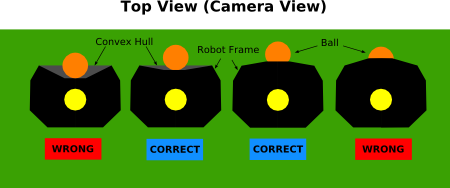
\includegraphics[width=1.0\columnwidth]{img/dribblers_above_view.png}
	\caption{The 80/20 ball covering/holding rule}
	\label{fig:20-rule}
\end{figure}

\item
A robot begins dribbling when it makes contact with the ball and stops dribbling when there is an observable separation between the ball and the robot.

The restriction on dribbling distance was added to prevent a robot with a mechanically superior dribbler having unchallenged control of the ball.
The distance restriction still allows dribblers to be used to aim and receive passes, turn around with the ball, and stop with the ball.
Dribblers can still be used to dribble large distances with the ball as long as the robot periodically loses possession, such as kicking the ball ahead of it as human soccer players often do.
The technical committee expects the distance rule to be self-enforced, i.e., teams will \removed{i}\added{e}nsure their software complies beforehand and may be asked to demonstrate this prior to a competition.
Referees, though, will still call fouls for violations and may give a caution (yellow card) for situations of repeated violations.

\item
The limitation to kicking speed was added to prevent a robot with a mechanically superior kicker from having too great of an advantage over opponents, or kicking the ball at speed unsafe for spectators.
It is also believed that this will help encourage team play over single robot ability, in a similar way to the restrictions on dribbling.

\item
The current rule about scoring after chip kicks is defined in this section (subsection Indirect Free Kicks) only.
During past competitions, some confusions occurred after robots chipped the ball and thereby caused own goals.
For this reason, a strict interpretation of this rule is provided here:
\begin{itemize}
\item \removed{I}\added{i}f a robot chips the ball (no matter at which height it travels) at a team mate and the ball subsequently enters the own goal, the opponent team scores\removed{.}
\item \removed{I}\added{i}f a robot chips the ball at an opponent and the ball subsequently enters the own goal while staying below 150\added{\,}mm all the time after touching the opponent robot, the opponent team also scores\removed{.}
\item \removed{I}\added{i}f a robot chips the ball at an opponent and the ball subsequently enters the own goal after having been above 150\added{\,}mm for some time (and not being in constant touch with the ground afterwards) after touching the opponent robot, the opponent team does not score\removed{.}
\end{itemize}

\item
The offence on deliberately entering the referee walking area was added to discourage teams from driving through this area to gain tactical advantages.
In particular, it should prevent teams from exploiting the fact that other teams might not have vision coverage of the referee walking area.
It is understood that on occasion a robot can enter the area if it is out of control\removed{,} or if it has been pushed into this area.
Such cases should not be considered offences.
However, the final decision as to what constitutes a deliberate violation is left to the referee.

\item
If a tipped over or broken robot does not constitute danger to other robots or humans, neither gives its team unfair advantage, the referee shall allow the game to continue until another game stoppage condition occurs.
The final decision as to what constitutes danger or unfair advantage is left to the referee.
\end{enumerate}

\section{Free Kicks}\label{sec:free-kicks}

\subsection{Types of Free Kicks}
Free kicks are either direct or indirect.

For both direct and indirect free kicks, the ball must be stationary when the kick is taken and the kicker does not touch the ball a second time until it has touched another robot.

\subsection{The Direct Free Kick}
\begin{itemize}
\item if a direct free kick is kicked directly into the opponents' goal, a goal is awarded to the
kicking team
\item if a direct free kick is kicked directly into the team's own goal, a corner kick is awarded
to the
opposing team
\end{itemize}

\subsection{The Indirect Free Kick}
A goal can be scored only if the ball subsequently touches another robot before it enters the goal.

\begin{itemize}
\item if an indirect free kick is kicked directly into the opponents' goal, a goal kick is awarded
to the opposing team.
\item if an indirect free kick is kicked directly into the team's own goal, a corner kick is
awarded to the opposing team.
\end{itemize}

\subsection{Free Kick Procedure}
If the free kick is awarded to a team inside \added{or within 200\,mm of} its own defence area, the free kick is taken from a point 600\,mm from the goal line and 100\,mm from the touch line closest to where the infringement occurred.

If the free kick is awarded to the attacking team within 700\,mm of the opposing defence area, the ball is moved to the closest point 700\,mm from the defence area.

Otherwise, the free kick is taken from the place where the infringement occurred.

All opponent robots are at least 500\,mm from the ball.

The ball is in play when it is kicked and moves.

\subsection{Infringements/Sanctions}
If, when a free kick is taken, an opponent is closer to the ball than the required distance:
\begin{itemize}
\item the kick is retaken
\end{itemize}

Any infringement as listed in \autoref{sec:ball-in-and-out-of-play} is handled accordingly.

For any other infringement of this Law:
\begin{itemize}
\item the kick is retaken
\end{itemize}

\section{The Penalty Kick}\label{sec:penalty-kick}

A penalty kick is awarded against a team which commits one of the five offences for which a direct free kick is awarded, inside its own defence area and while the ball is in play.

A goal may be scored directly from a penalty kick.

Additional time is allowed for a penalty kick to be taken at the end of each half or at the end of periods of extra time.

\subsection{Position of the Ball and the Robots}
The ball:

\begin{itemize}
\item is placed on the penalty mark
\end{itemize}

The robot taking the penalty kick:

\begin{itemize}
\item is properly identified
\end{itemize}

The defending goalkeeper:

\begin{itemize}
\item remains between the goalposts, touches its goal line, and faces outward of the goal, until the ball has been kicked; it is allowed to move before the ball has been kicked, as long as its motion does not break any of these constraints
\end{itemize}

The robots other than the kicker are located:

\begin{itemize}
\item inside the field of play
\item behind a line parallel to the goal line and 400\,mm behind the penalty mark
\end{itemize}

\subsection{The Referee}
\begin{itemize}
\item does not signal for a penalty kick to be taken until the robots have taken up position in accordance with the Law
\item decides when a penalty kick has been completed
\end{itemize}

\subsection{Procedure}
\begin{itemize}
\item the robot taking the penalty kicks the ball forward
\item it does not play the ball a second time until it has touched another robot
\item the ball is in play when it is kicked and moves forward
\end{itemize}

When a penalty kick is taken during the normal course of play, or time has been extended at half-time or full time to allow a penalty kick to be taken or retaken, a goal is awarded if, before passing between the goalposts and under the crossbar:

\begin{itemize}
\item the ball touches either or both of the goalposts and/or the crossbar, and/or the goalkeeper
\end{itemize}

\subsection{Infringements/Sanctions}
\textit{If the referee gives the signal for a penalty kick to be taken and, before the ball is in play, one of the following situations occurs:}

The robot taking the penalty kick infringes the Laws of the Game:

\begin{itemize}
\item the referee allows the kick to proceed
\item if the ball enters the goal, the kick is retaken
\item if the ball does not enter the goal, the kick is not retaken
\end{itemize}

The goalkeeper infringes the Laws of the Game:

\begin{itemize}
\item the referee allows the kick to proceed
\item if the ball enters the goal, a goal is awarded
\item if the ball does not enter the goal, the kick is retaken
\end{itemize}

A team-mate of the robot taking the kick enters the area 400\,mm behind the penalty mark:

\begin{itemize}
\item the referee allows the kick to proceed
\item if the ball enters the goal, the kick is retaken
\item if the ball does not enter the goal, the kick is not retaken
\item if the ball rebounds from the goalkeeper, the crossbar or the goal post and is touched by this robot, the referee stops play and restarts the match with an indirect free kick to the defending team
\end{itemize}

A team-mate of the goalkeeper enters the area 400\,mm behind the penalty mark:

\begin{itemize}
\item the referee allows the kick to proceed
\item if the ball enters the goal, a goal is awarded
\item if the ball does not enter the goal, the kick is retaken
\end{itemize}

A robot of both the defending team and the attacking team infringe the Laws of the Game:

\begin{itemize}
\item the kick is retaken
\end{itemize}

\textit{If, after the penalty kick has been taken:}

Any infringement as listed in \autoref{sec:ball-in-and-out-of-play} is handled accordingly.

The ball is touched by an outside agent as it moves forward:

\begin{itemize}
\item the kick is retaken
\end{itemize}

The ball rebounds into the field of play from the goalkeeper, the crossbar or the goalposts, and is then touched by an outside agent:

\begin{itemize}
\item the referee stops play
\item play is restarted with a dropped ball at the place where it touched the outside agent (see \autoref{sec:free-kicks})
\end{itemize}

\section{The Throw-In}\label{sec:throw-in}

A throw-in is a method of restarting play.

A goal cannot be scored directly from a throw-in.

A throw-in is awarded:

\begin{itemize}
\item when the whole of the ball passes over the touch boundary, either on the ground or in the air
\item from the point 100\,mm perpendicular to the touch boundary where the ball crossed the touch boundary
\item to the opponents of the robot that last touched the ball
\end{itemize}

\subsection{Procedure}
\begin{itemize}
\item the referee places the ball at the designated position
\item all opponent robots are at least 500\,mm from the ball
\item the ball is in play when it is kicked and moves
\end{itemize}

\subsection{Infringements/Sanctions}
If, when a throw-in is taken, an opponent is closer to the ball than the required distance:

\begin{itemize}
\item the throw-in is retaken
\end{itemize}

Any infringement as listed in \autoref{sec:ball-in-and-out-of-play} is handled accordingly.

For any other infringement:

\begin{itemize}
\item the kick is retaken
\end{itemize}

\section{The Goal Kick}\label{sec:goal-kick}

A goal kick is a method of restarting play.

A goal may be scored directly from a goal kick, but only against the opposing team.

A goal kick is awarded when:

\begin{itemize}
\item the whole of the ball, having last touched a robot of the attacking team, passes over the goal line, either on the ground or in the air, and a goal is not scored in accordance with \autoref{sec:method-of-scoring}
\end{itemize}

\subsection{Procedure}
\begin{itemize}
\item the ball is kicked from a point 500\,mm from the goal line and 100\,mm from the touch line closest to where the ball passed over the goal boundary
\item opponents remain 500\,mm from the ball until the ball is in play
\item the kicker does not play the ball a second time until it has touched another robot
\item the ball is in play when it is kicked and moves
\end{itemize}

\subsection{Infringements/Sanctions}
Any infringement as listed in \autoref{sec:ball-in-and-out-of-play} is handled accordingly\added{.}

For any other infringement of this Law:
\begin{itemize}
\item the kick is retaken
\end{itemize}

\section{The Corner Kick}\label{sec:corner-kick}

A corner kick is a method of restarting play.

A goal may be scored directly from a corner kick, but only against the opposing team.

A corner kick is awarded when:

\begin{itemize}
\item the whole of the ball, having last touched a robot of the defending team, passes over the goal line, either on the ground or in the air, and a goal is not scored in accordance with \autoref{sec:method-of-scoring}
\end{itemize}

\subsection{Procedure}
\begin{itemize}
\item the ball is kicked from the nearest corner, 100\,mm in from both the goal line and the touch line
\item opponents remain 500\,mm from the ball until the ball is in play
\item the kicker does not play the ball a second time until it has touched another robot
\item the ball is in play when it is kicked and moves
\end{itemize}

\subsection{Infringements/Sanctions}
Any infringement as listed in \autoref{sec:ball-in-and-out-of-play} is handled accordingly.

For any other infringement:

\begin{itemize}
\item the kick is retaken
\end{itemize}


\appendix

\section{The Competition Rules}\label{app:competition-rules}

This appendix describes additional procedures for Small Size League matches.

\subsection{Extra Time}
If the game is drawn after the end of the second period and the game needs to end with a clear winner, extra time will be played (as stated in laws 7 and 10).
Before the first half of extra time, there will be an interval that must not exceed 5 minutes.

\subsubsection{Periods of Play in Extra Time}
The extra time lasts two equal periods of 5 minutes, unless otherwise mutually agreed between the referee and the two participating teams.
Any agreement to alter the periods of extra time (for example, to reduce each half to 3 minutes because of a limited schedule) must be made before the start of play and must comply with competition rules.

\subsubsection{Extra Time Half-Time Interval}
Teams are entitled to an interval at half-time.
The half-time interval must not exceed 2 minutes.
The duration of the half-time interval may be altered only with the consent of both teams and the referee.

\subsubsection{Timeouts}
Each team is allocated two timeouts at the beginning of extra time.
A total of 5 minutes is allowed for all timeouts.
The number of timeouts and the time not used in regular game are not added.
Timeouts in extra time follow the same rules as in regular game (stated in \autoref{sec:duration-of-the-match}).

\subsection{Penalty Shoot-Out}
If the game is drawn after the end of the second period of extra time, kicks from the penalty mark will be taken to decide which teams wins the game.

\subsubsection{Preparation}
Before the first penalty is kicked, there will be an interval that must not exceed 2 minutes.
This time is suggested to be used by the teams in dialogue with the referee and his assistants to check whether the goalie's position is correct (on the line) and all other rules for penalty can be fullfilled as stated in \autoref{sec:penalty-kick}.
The referee determines (e.g., by flipping a coin) which team defends which goal as well as which team has to take the first penalty kick.

\subsubsection{Procedure}
During the kicks from the penalty mark, a maximum of 2 robots per team is on the field in order to avoid interference.
The kicks from the penalty mark are taken alternately by the teams until each team has kicked 5 penalties.
If a decision is reached for one team, the kicks are stopped by the referee.
For all penalties, the rules of \autoref{sec:penalty-kick} apply.
A second kick (e.g., if the ball bounces back from the goalie or a goalpost) or a bounce back from the kicker will not score; as soon as the kicker touches the ball after he released it the first time the penalty is over.
During the kicks from the penalty mark no timeout is possible.
Robots may be exchanged between the kicks following the interchange rules of \autoref{sec:number-of-robots}.
As switching sides would cost too much time and would force the teams to touch their systems both goals are used.

If after 10 kicks no decision is reached, each team takes another penalty in the same order as before.
This procedure (one penalty each team) is continued until a decision is reached.

\subsection{Abandoned Match}
If one of the teams abandons the match, before or during its course, the opponent will be awarded winner for all purposes.
However, solely for the purpose of goal difference counting, the winner team can, at its decision, continue to play by itself, and the goals scored will continue to be computed.

If the two teams abandon the match, before or during its course, both teams are considered to have lost the match.
Abandoned matches cannot result in ties.

The competition records will indicate the team(s) that abandoned the match.

\added{A team that refuses to make a good faith effort to participate in a
scheduled game will be disqualified from the competition.}

\subsection{Early Termination of Match at Score of 10}

When the score difference reaches 10 goals in a round-robin (not tournament) game, the match is automatically terminated and the team with more goals declared the winner.

\subsection{Round-Robin Ranking Criteria}

During the round-robin phase of the competition, the ranking of each team in each group will be determined by the following criteria, in order:
\begin{itemize}
\item greatest number of points obtained in all group matches
\item goal difference in all group matches
\item greatest number of goals scored in all group matches
\end{itemize}

\subsubsection{Tiebreaking}
If two or more teams are equal on the basis of the above criteria, the tiebreaking procedure to determine their rankings will be determined by the following criteria, in order:
\begin{itemize}
\item greatest number of points obtained in the group matches between the teams concerned
\item goal difference resulting from the group matches between the teams concerned
\item greater number of goals scored in all group matches between the teams concerned
\item drawing of lots by the Organising Committee
\end{itemize}

\section{Appendix B - Vision Experts}\label{app:vision-experts}

During competitions, vision experts are in charge of the shared vision systems on each field.
The assignment and timing of their service period is allocated by competition organisers.
This must be done in a way that each shared vision system always has at least one vision expert assigned.

\subsection{Duties}
The Vision Expert:
\begin{itemize}
\item checks shared vision system hardware and reports any kind of hardware problems to TC members / local organisers
\item does the SSL-Vision calibration procedure whenever needed or when teams request, during setup times
\item does the SSL-Vision calibration or maintenance during a match when referee requests
\item before each match, checks that both teams can receive the SSL-Vision packets properly
\item before each match, checks that both teams use proper standard patterns, that their robot heights are calibrated accurately, and that their received localization data is correct
\item monitors shared vision system status during the match and reports any kind of problems to the referee instantly
\item receives complaints from teams about shared vision system during the match and, if needed, asks the referee to halt the game to give time to diagnose and fix the problem
\item notifies the referee if there is a non-resolvable complaint from a team regarding the vision system; in this case, the referee has the final authority to rule in any manner within his powers and duties (see \autoref{sec:referee}), including the ability to warn and/or sanction a team for unsporting behavior if the team's requests are unfounded and continue to obstruct the game (see \autoref{subsec:fouls-and-misconduct-disciplinary-sanctions}).
\end{itemize}

\end{document}
